\chapter{Dostupnost, distribuce a~použití PROTOPlantu}
Jak popisuji v~úvodu, jedním z~cílů, který jsem si dal na začátku práce na PROTOPlantu, bylo šíření pod licencí open-source.
Toto jsem dodržel. 
Celý software PROTOPlantu je šířen pod licencí MIT, ostatní části (hardware, atd.) včetně textu této práce je poté pod CC BY-NC-SA 4.0.
Přitom převzatý hardware (senzory, procesor a další moduly) je z~licence vyňat.

Člověk, který elektrotechnice a programování rozumí, si poté může PROTOPlant bez problému sestavit sám v~pohodlí domova.

Ovšem stále je obrovské množství lidí, kteří na sestavení PROTOPlantu nemusí mít dostatečné znalosti, nebo nemají čas si jej sestavovat.
Z~toho důvodu plánuji zahájit výrobu a distribuci mého systému jakožto hotových komponent, které stačí nainstalovat a zapojit.

Ke dni \It{20. 2. 2020} jsem ve fázi, kdy připravuji výrobní podklady jednotlivých komponent, a provádím kroky vedoucí k~založení podniku.
Již v~minulém roce jsem provedl průzkum, který ukázal, že o~PROTOPlant by skutečně byl zájem.

\section{Případové studie}
Pro názorný příklad použití PROTOPlantu uvádím konkrétní případové studie.

\subsection{Malý skleník s užitkovými rostlinami}
Zahrádkář pěstující plodiny čistě pro zásobování sebe a své rodiny čerstvou zeleninou vlastní skleník s plochou obdělávané půdy 6x3 metry.
Výška skleníku jsou přibližně dva metry, jeho objem je tedy vzhledem k tvaru skleníku \B{menší, než 36~m\superscript{3}}.
Pro dostatečné pokrytí prostoru senzorikou zde stačí dva senzory teploty (viz kapitola \ref{sec:DS18B20}) a jeden senzor vzdušné vlhkosti (viz kapitola \ref{sec:DHT22}). 
Vzhledem k obdělávané ploše, stačí použít 4 senzory půdní vlhkosti.
Zavlažování je vzhledem k pěstovaným rostlinám řešeno děrovanou hadicí položenou přímo na půdě.
Berme v potaz, že zahrádkář chce, aby PROTOPlant otevíral jen jedno okno.
Vzhledem k velikosti okna postačí aktuátor s délkou výsuvu 20~cm.

\fxnote[author=PŠ]{Zde přibudou fotografie babiččina skleníku}

\begin{table}[h]
    \centering
    \resizebox{\textwidth}{!}{%
    \begin{tabular}{llll}
    \multicolumn{1}{l|}{\textbf{Položka}}            & \textbf{Počet kusů} & \multicolumn{1}{l|}{\textbf{Cena za kus}} & \textbf{Cena celkem} \\ \hline
    \multicolumn{1}{l|}{Řídící jednotka}             & 1                   & \multicolumn{1}{l|}{1800 Kč}              & 1800 Kč              \\
    \multicolumn{1}{l|}{Aktuátory pro ovládání oken} & 1                   & \multicolumn{1}{l|}{700 Kč}               & 700 Kč               \\
    \multicolumn{1}{l|}{Senzory teploty}             & 2                   & \multicolumn{1}{l|}{60 Kč}                & 120 Kč               \\
    \multicolumn{1}{l|}{Senzor vzdušné vlhkosti}     & 1                   & \multicolumn{1}{l|}{60 Kč}                & 60 Kč                \\
    \multicolumn{1}{l|}{Senzor půdní vlhkosti}       & 4                   & \multicolumn{1}{l|}{25 Kč}                & 100 Kč               \\
    \multicolumn{1}{l|}{Kabely, hadice, spoj. mat.}  & 1                   & \multicolumn{1}{l|}{300 Kč}               & 300 Kč               \\
    \multicolumn{1}{l|}{Čerpadlo}                    & 1                   & \multicolumn{1}{l|}{800 Kč}               & 800 Kč               \\ \hline
    \B{Cena celkem}                                  &                     &                                           & \B{3880 Kč}          
    \end{tabular}%
    }
    \caption{Tabulka s cenovou kalkulací systému pro menší skleník.}
    \label{tab:SmallGreenhousePricing}
\end{table}

\subsection{Středně velký skleník s okrasnými rostlinami}
Skleník, ve kterém PROTOPlant průběžně testuji je určen pro pěstování orchidejí. 
Jeho plocha je přibližně 10~x~4~m.
Většina rostlin je v květináčích s molitanem či substrátem zavěšena v prostoru, nebo položena na stole.
Teplotní senzory jsou zde použity 4, senzory vlhkosti 3.
Vzhledem k tomu, že většina z těchto rostlin je epifytní, nesnášejí trvale vlhkou půdu. 
Z tohoto důvodu je zavlažování řešeno rozprašovačem umístěným pod stropem skleníku a upraveným nastavením jeho spínání.
Neprobíhá tedy tak často.

\begin{table}[h]
    \centering
    \resizebox{\textwidth}{!}{%
    \begin{tabular}{llll}
    \multicolumn{1}{l|}{\textbf{Položka}}            & \textbf{Počet kusů} & \multicolumn{1}{l|}{\textbf{Cena za kus}} & \textbf{Cena celkem} \\ \hline
    \multicolumn{1}{l|}{Řídící jednotka}             & 1                   & \multicolumn{1}{l|}{1800 Kč}              & 1800 Kč              \\
    \multicolumn{1}{l|}{Aktuátory pro ovládání oken} & 2                   & \multicolumn{1}{l|}{900 Kč}               & 1800 Kč              \\
    \multicolumn{1}{l|}{Senzory teploty}             & 3                   & \multicolumn{1}{l|}{60 Kč}                & 180 Kč               \\
    \multicolumn{1}{l|}{Senzor vzdušné vlhkosti}     & 2                   & \multicolumn{1}{l|}{60 Kč}                & 120 Kč               \\
    \multicolumn{1}{l|}{Senzor půdní vlhkosti}       & 2                   & \multicolumn{1}{l|}{25 Kč}                & 50 Kč                \\
    \multicolumn{1}{l|}{Kabely, hadice, spoj. mat.}  & 1                   & \multicolumn{1}{l|}{400 Kč}               & 400 Kč                \\
    \multicolumn{1}{l|}{Čerpadlo}                    & 1                   & \multicolumn{1}{l|}{800 Kč}               & 1000 Kč              \\ \hline
    \B{Cena celkem}                                  &                     &                                           & \B{5350 Kč}             
    \end{tabular}%
    }
    \caption{Tabulka s cenovou kalkulací systému pro větší skleník.}
    \label{tab:MedGreenhousePricing}
\end{table}

\begin{figure}[htbp]
    \centering
    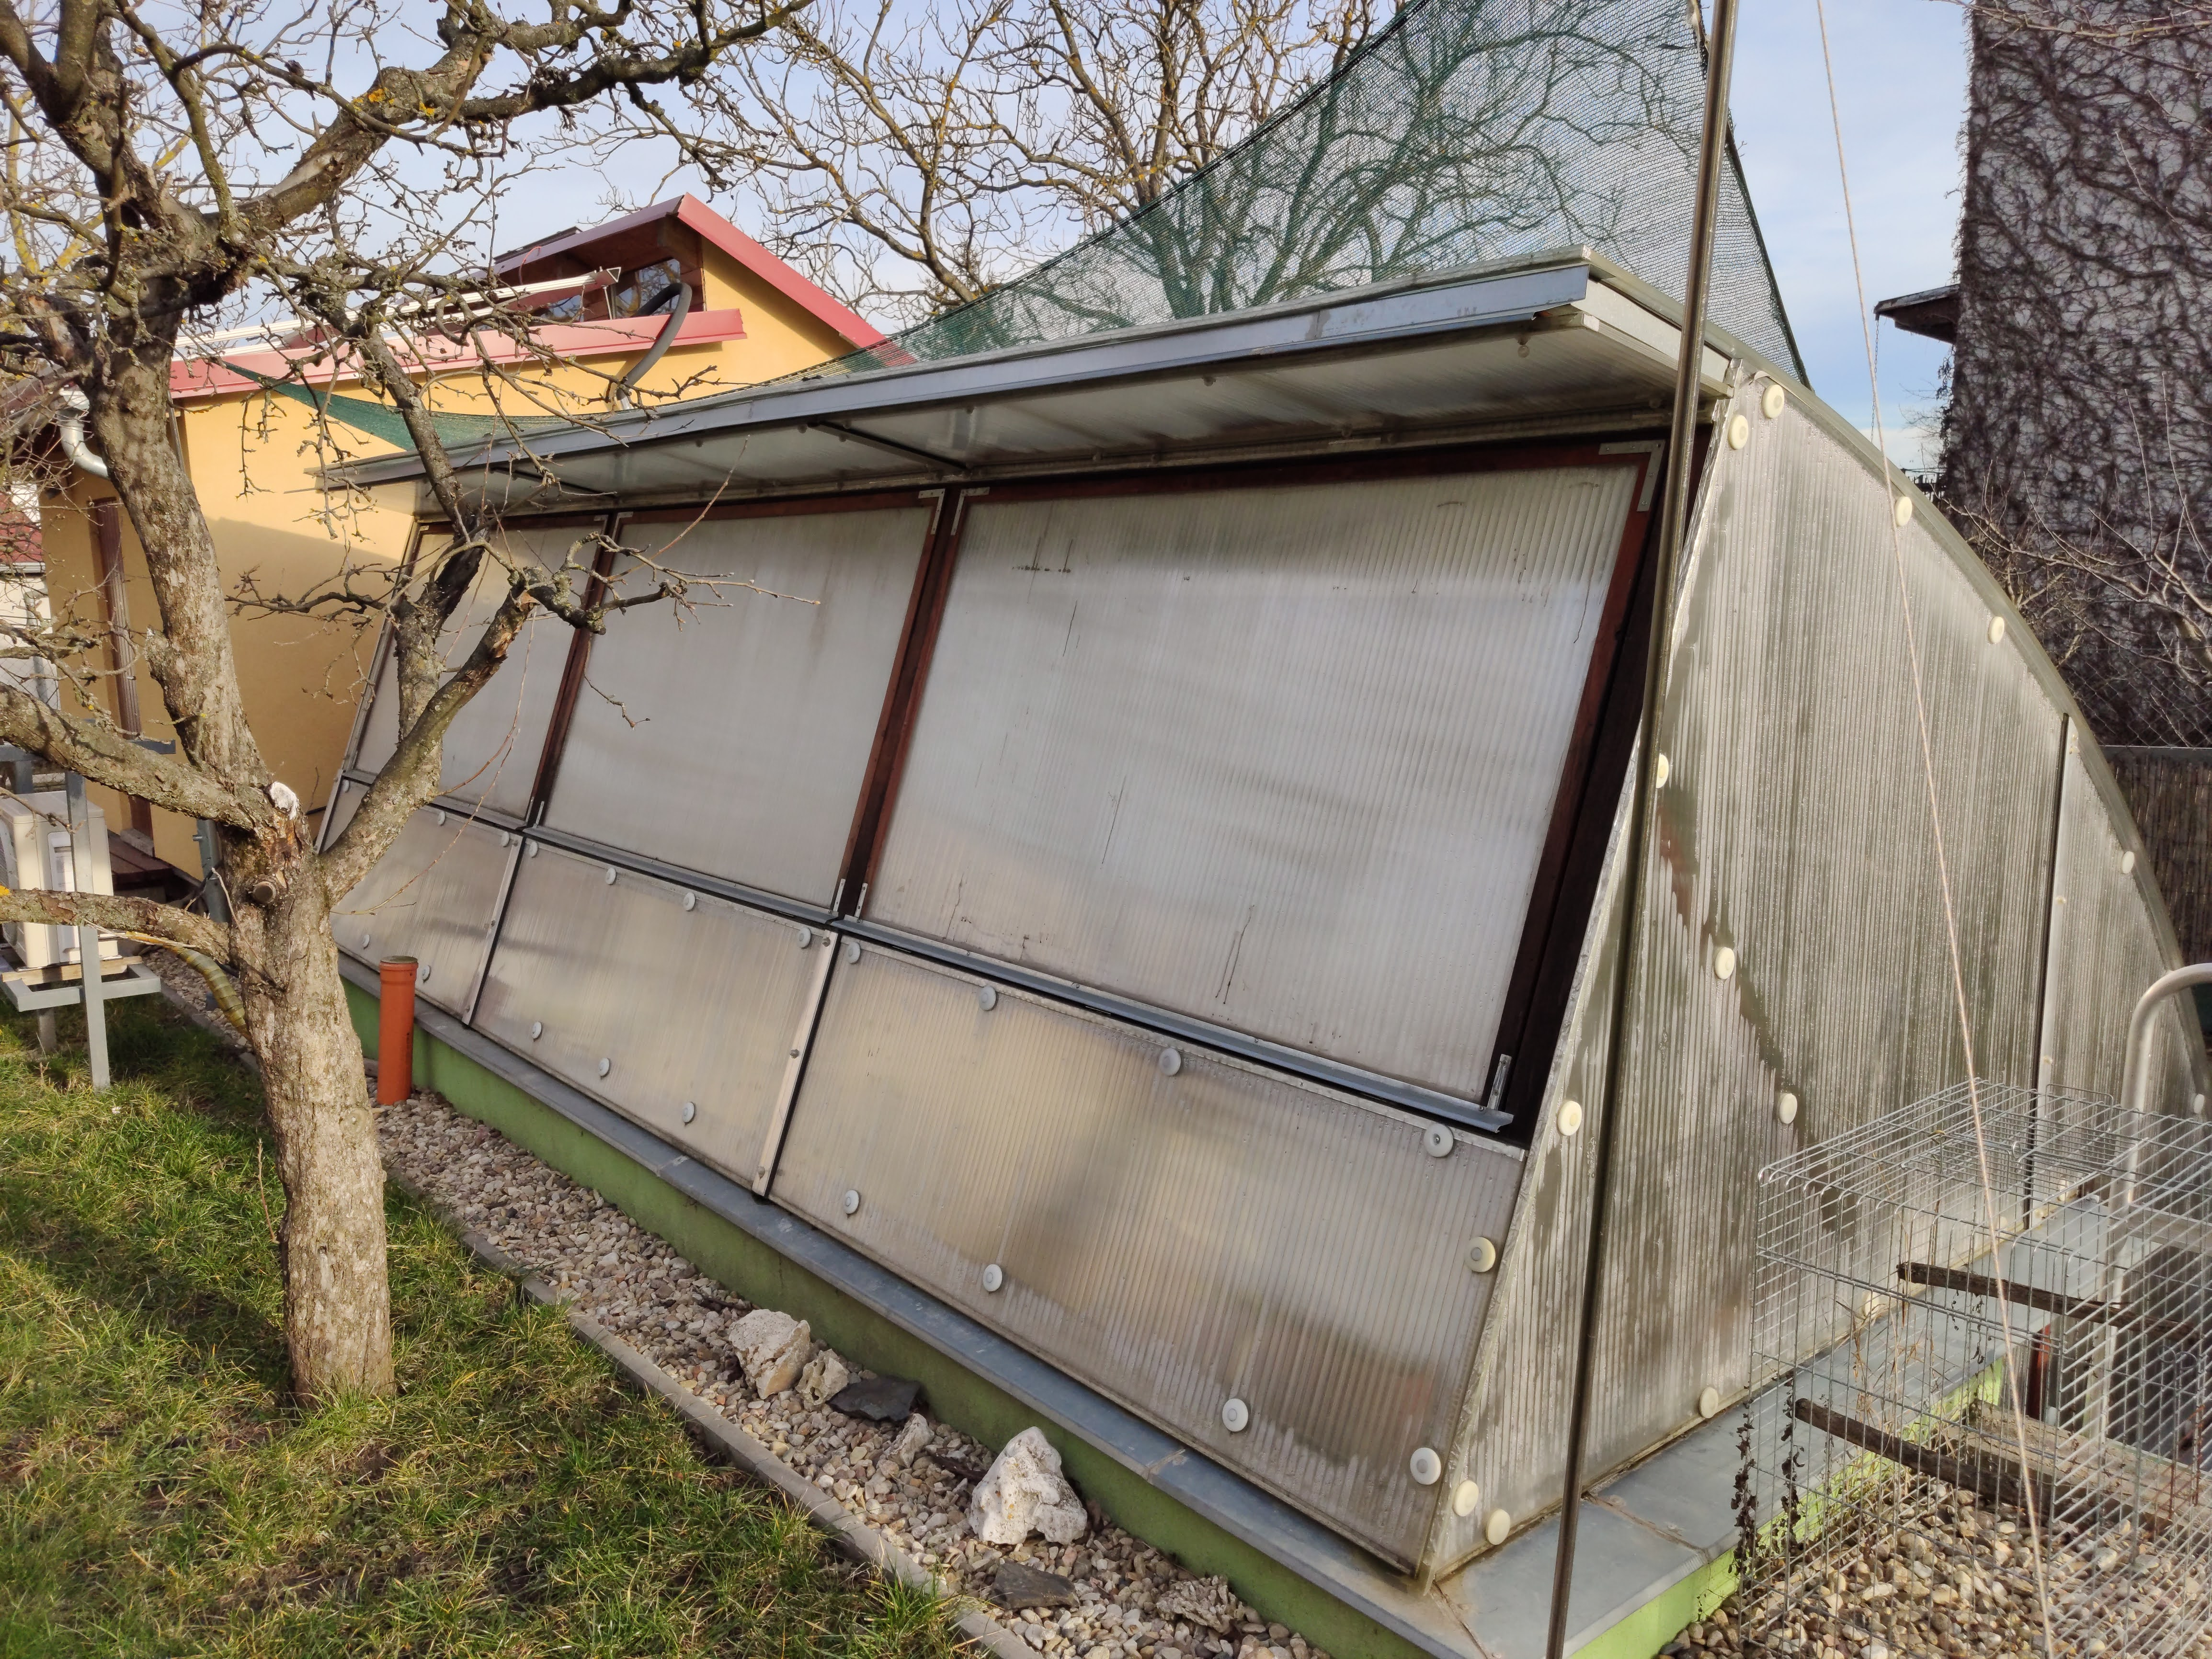
\includegraphics[width=\textwidth]{img/PHOTOS/OrchidHouse_EXTERIOR.jpg}
    \caption{Exteriér testovacího skleníku}
    \label{fig:OrchidHouse_EXTERIOR}
\end{figure}

\begin{figure}[htbp]
    \centering
    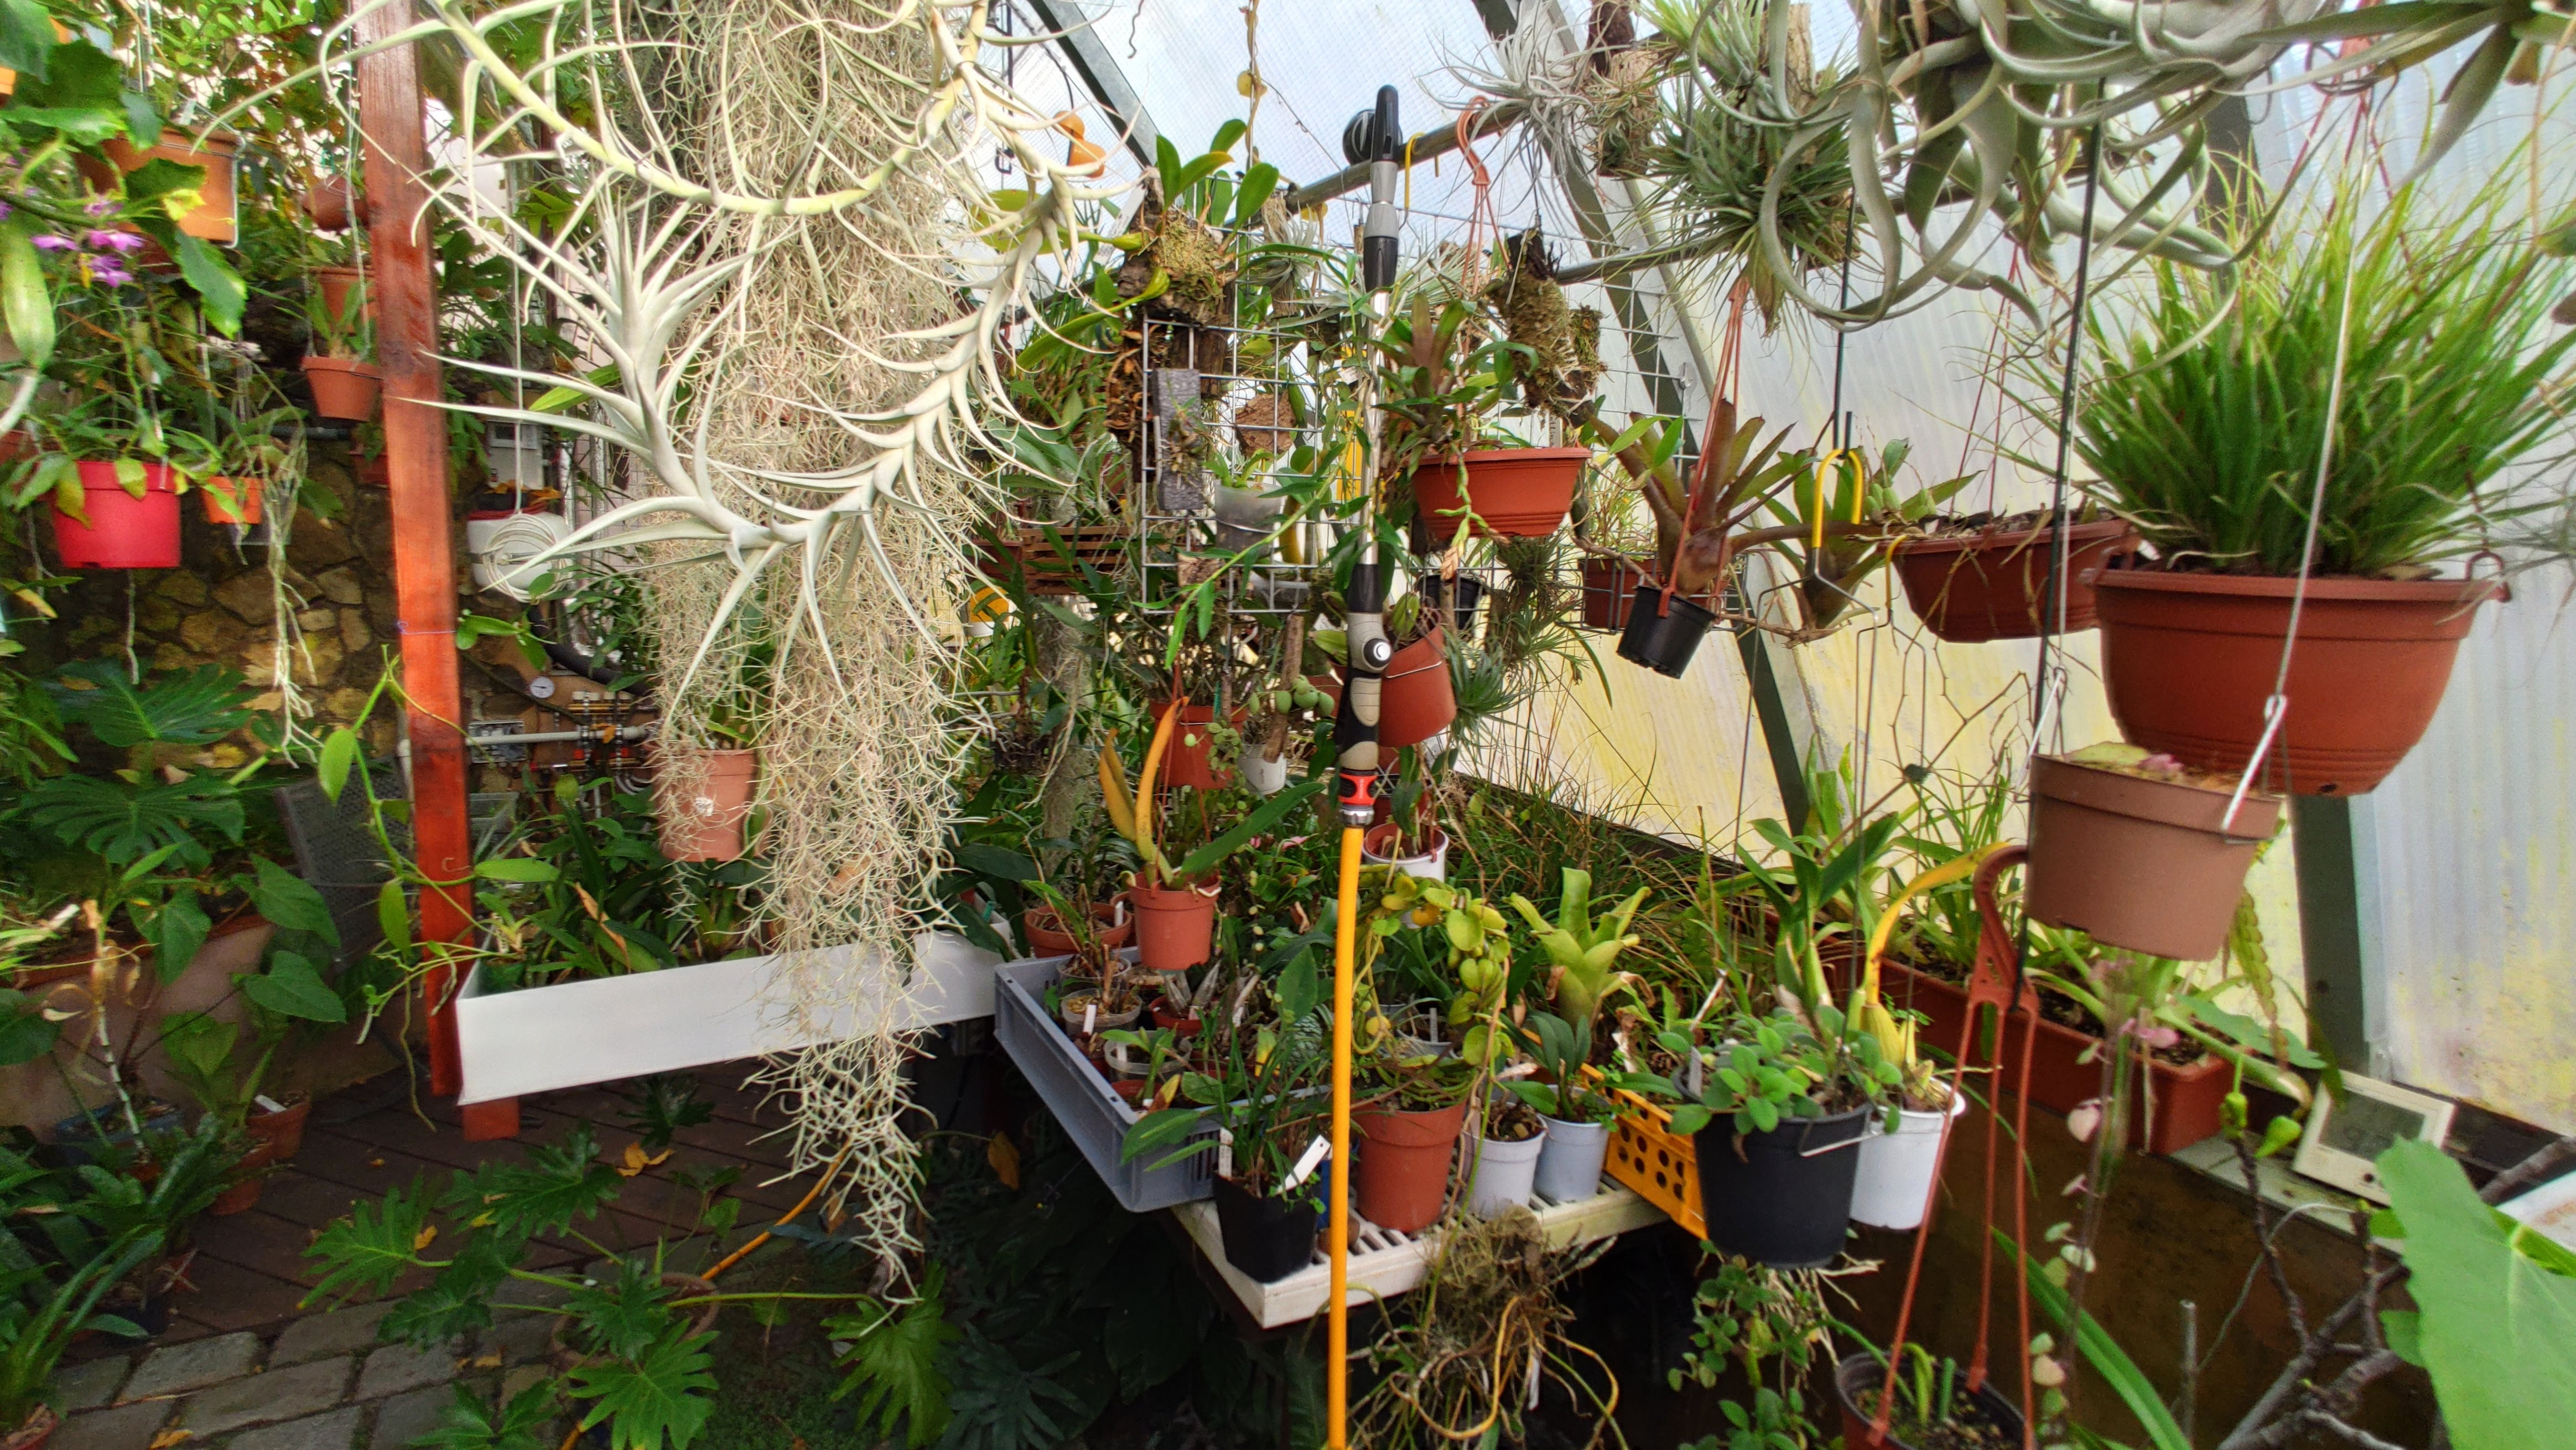
\includegraphics[width=\textwidth]{img/PHOTOS/OrchidHouse_INTERIOR.jpg}
    \caption{Interiér testovacího skleníku}
    \label{fig:OrchidHouse_INTERIORs}
\end{figure}
\newpage